% Options for packages loaded elsewhere
\PassOptionsToPackage{unicode}{hyperref}
\PassOptionsToPackage{hyphens}{url}
%
\documentclass[
]{article}
\usepackage{amsmath,amssymb}
\usepackage{lmodern}
\usepackage{ifxetex,ifluatex}
\ifnum 0\ifxetex 1\fi\ifluatex 1\fi=0 % if pdftex
  \usepackage[T1]{fontenc}
  \usepackage[utf8]{inputenc}
  \usepackage{textcomp} % provide euro and other symbols
\else % if luatex or xetex
  \usepackage{unicode-math}
  \defaultfontfeatures{Scale=MatchLowercase}
  \defaultfontfeatures[\rmfamily]{Ligatures=TeX,Scale=1}
  \setmainfont[]{Arial}
\fi
% Use upquote if available, for straight quotes in verbatim environments
\IfFileExists{upquote.sty}{\usepackage{upquote}}{}
\IfFileExists{microtype.sty}{% use microtype if available
  \usepackage[]{microtype}
  \UseMicrotypeSet[protrusion]{basicmath} % disable protrusion for tt fonts
}{}
\makeatletter
\@ifundefined{KOMAClassName}{% if non-KOMA class
  \IfFileExists{parskip.sty}{%
    \usepackage{parskip}
  }{% else
    \setlength{\parindent}{0pt}
    \setlength{\parskip}{6pt plus 2pt minus 1pt}}
}{% if KOMA class
  \KOMAoptions{parskip=half}}
\makeatother
\usepackage{xcolor}
\IfFileExists{xurl.sty}{\usepackage{xurl}}{} % add URL line breaks if available
\IfFileExists{bookmark.sty}{\usepackage{bookmark}}{\usepackage{hyperref}}
\hypersetup{
  pdftitle={La raport intermédiaire},
  pdfauthor={Antoine Viguié, Aymane Berriane, Christian Alvarez Leon, Meng Wang, Yu PENG},
  hidelinks,
  pdfcreator={LaTeX via pandoc}}
\urlstyle{same} % disable monospaced font for URLs
\usepackage[margin=1in]{geometry}



\usepackage{longtable,booktabs,array}
\usepackage{calc} % for calculating minipage widths
% Correct order of tables after \paragraph or \subparagraph
\usepackage{etoolbox}
\makeatletter
\patchcmd\longtable{\par}{\if@noskipsec\mbox{}\fi\par}{}{}
\makeatother
% Allow footnotes in longtable head/foot
\IfFileExists{footnotehyper.sty}{\usepackage{footnotehyper}}{\usepackage{footnote}}
\makesavenoteenv{longtable}


\setlength{\emergencystretch}{3em} % prevent overfull lines
\providecommand{\tightlist}{%
  \setlength{\itemsep}{0pt}\setlength{\parskip}{0pt}}
\setcounter{secnumdepth}{5}
\usepackage{booktabs}
\usepackage{amsthm}

%使用中文要使用这个包
\usepackage{ctex}

\usepackage{graphicx}
\graphicspath{{images/}} %表示图片在当前目录下的images目录

%封面====================================================================================================================
\usepackage{pdfpages}
%=========================================================================================================================

%重新命名=================================================================================================================

%\renewcommand{\bibname}{你的BIBLIOGRAPHY}
%\renewcommand{\abstractname}{你的ABSTRACT}

\renewcommand{\refname}{RÉFERENCES}

%\renewcommand{\chaptername}{Chapitre}

%\usepackage{titlesec}

%\usepackage{lipsum}

%\titleformat{\chapter}[display]{\normalfont\bfseries}{}{0pt}{\Large}

%标题命名
\renewcommand{\contentsname}{SOMMAIRE}

%图命名
\renewcommand{\figurename}{Figure}

%在toc中包含reference :https://tex.stackexchange.com/questions/57427/how-to-add-printindex-to-tableofcontents
\usepackage{makeidx}
\makeindex
\usepackage[nottoc]{tocbibind}

%toc 没有headers页眉
\addtocontents{toc}{\protect\thispagestyle{empty}}

%=========================================================================================================================


%页眉页脚==================================================================================================================

%\fancyhead[R]{\kaishu 中国矿业大学~(北京) 硕士学位论文}
%\lhead{page \thepage\ of \pageref{LastPage}}
%\fancyhead[RO,LE]{\CJKfamily{hei} \bfseries \LaTeX{} 排版系统}
%\fancyhead[LO,RE]{\CJKfamily{hei>} \bfseries \leftmark}
%\renewcommand{\headrule}{\hrule width\headwidth \vspace{1.5pt}\hrule width\headwidth} % 所谓的文武线



%定义页眉页脚 fancyhdr 包
\usepackage{fancyhdr}

\pagestyle{fancy}

%默认清除所有的页眉和页脚设置
\fancyhf{} %清空页眉页脚 这是个更底层的命令

%设置页眉高度
\setlength\headheight{40pt}

%多行
%\fancyhead[c]{From: Frank\\To: Michel}

% 使用tabular 多行对齐
% \rhead{
    % \begin{tabular}[b]{l@{}}
        % Page: \thepage\\\today
    % \end{tabular}
    % }
\lhead{
\includegraphics[height=30pt]{ecole.png}}
\rfoot{\thepage}

%页眉横线
%\renewcommand\headrulewidth{0pt} %隐藏页眉横线
\renewcommand{\headrule}{\hrule width\headwidth \vspace{1.5pt}\hrule width\headwidth} % 所谓的文武线

%==========================================================================================================================

\makeatletter
\def\thm@space@setup{%
  \thm@preskip=8pt plus 2pt minus 4pt
  \thm@postskip=\thm@preskip
}
\makeatother

% 让url连接变为脚注
\renewcommand{\href}[2]{#2\footnote{\url{#1}}}

% 浮动

\usepackage{float}
\usepackage{float}
\ifluatex
  \usepackage{selnolig}  % disable illegal ligatures
\fi

%natbib 选项======================================================================================================

\usepackage[]{natbib}
\bibliographystyle{plainnat}



\title{La raport intermédiaire}
\author{Antoine Viguié, Aymane Berriane, Christian Alvarez Leon, Meng Wang, Yu PENG}
\date{2020-12-08}

%==========================================================================================================================================

\begin{document}


%插入封面=================================================================
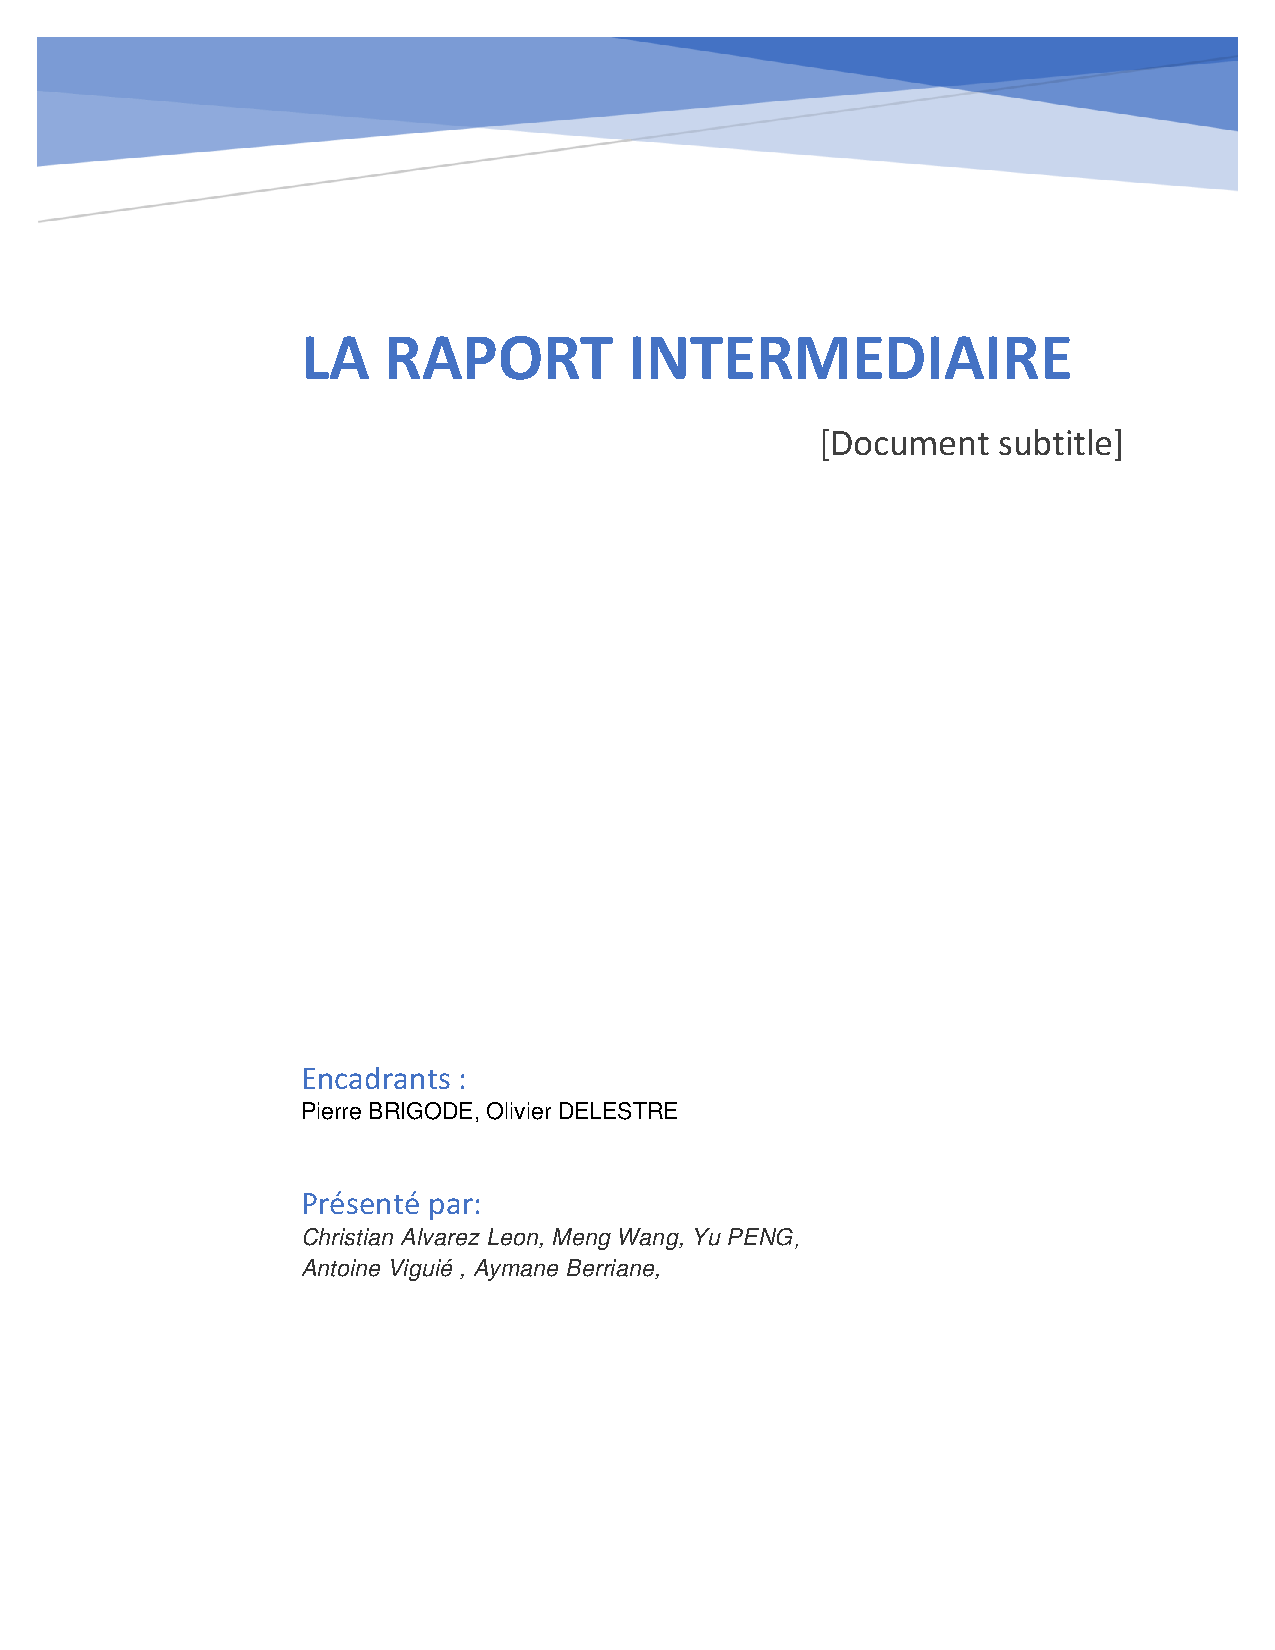
\includepdf{images/COVERPAGE.pdf}
%=======================================================================

%插入标题=================================================================
%%%\maketitle
%%=======================================================================

%加空白页但又heater
%\newpage
%\mbox{}
%\newpage



{
\setcounter{tocdepth}{2}
\tableofcontents
}


\newpage

\hypertarget{introduction}{%
\section*{Introduction}\label{introduction}}
\addcontentsline{toc}{section}{Introduction}

On observe régulièrement sur la Côte d'Azur, notamment à l'automne, de forts épisodes pluvieux, pouvant engendrer des crues. Par exemple, le 23 novembre 2019, des inondations exceptionnelles se sont produites sur la Côte d'Azur et ont inondé les plaines alluviales de l'Argens, de la Siagne et de la Brague notamment. Plus récemment, début octobre 2020, les vallées de la Roya, de la Vésubie ont été ravagées par des inondations, avec 500 mm relevés pendant l'épisode à Saint-Martin-Vésubie \citep{noauthor_meteo-france_nodate}, du jamais vu à cette station depuis les relevés météorologiques. En raison de la nature destructrice des inondations, des recherches hydrologiques sur les bassins versants doivent être menées pour prendre les mesures d'anticipation et de protection de la population. Ceci nécessite par exemple de mesurer le débit sur des sections de cours d'eau non instrumentées en appareils de mesure. Dans notre projet, le but est de calculer le débit d'une section du canal de la Siagne par le logiciel Fudaa-LSPIV. Celui-ci permet de traiter des séquences d'images ou des vidéos d'écoulements pour calculer les champs de vitesse de surface et débit de la section choisie. Ce logiciel peut s'avérer utile pour mesurer le débit de sections de rivières avec un fort courant et de nombreux objets flottants, car les méthodes classiques seraient susceptibles d'abîmer le matériel. Il s'avèrera aussi nécessaire d'utiliser une autre méthode de mesure de débit, comme l'ADCP, pour comparer les résultats obtenus.

\newpage

\hypertarget{contexte-du-projet}{%
\section{Contexte du projet}\label{contexte-du-projet}}

\hypertarget{zone-daction}{%
\subsection{Zone d'action}\label{zone-daction}}

Le canal de la Siagne permet d'acheminer l'eau prélevée dans la Siagne depuis Saint-Cézaire-sur-Siagne jusqu'à Cannes sur un parcours de 50 km (figure \ref{fig:refsiagne}). La section étudiée est située à Mougins, dans le département des Alpes-Maritimes (figure 2).



\begin{figure}[H]
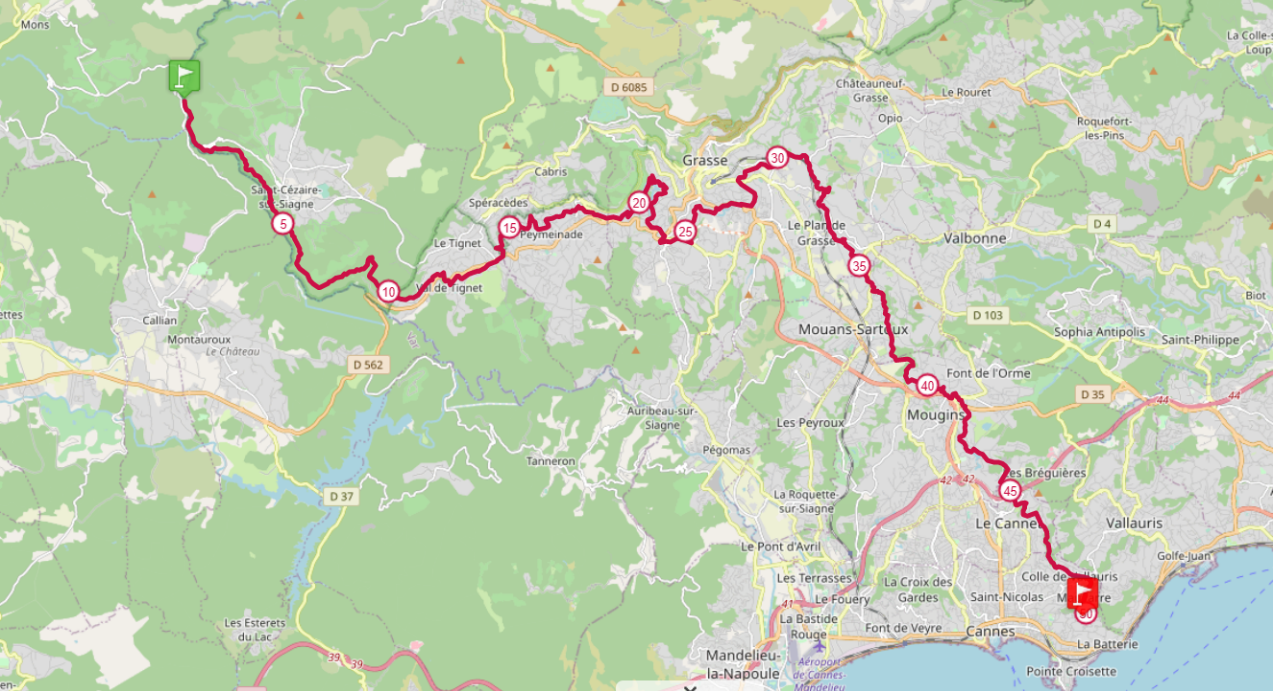
\includegraphics[width=1\linewidth,]{images/siagne} \caption{Localisation géographique du canal de la Siagne (tracedetrail.fr)}\label{fig:refsiagne}
\end{figure}

Datant de 1868, c'est un ouvrage hydraulique de transport et d'alimentation en eau vers la ville de Grasse ainsi que Cannes et ses environs.
Désormais élément du paysage local, le canal s'étend à ciel ouvert sur une grande partie.
La section étudiée est facilement accessible à pieds comme en voiture, ce qui facilite les mesures. Puis, la forme du canal est simple et le débit faible, ce qui donnera une mesure de débit plus précise \citep{noauthor_canaldelasiagnefr_2019}.

\hypertarget{pruxe9sentation-des-muxe9thodes-lspiv}{%
\subsection{Présentation des méthodes LSPIV}\label{pruxe9sentation-des-muxe9thodes-lspiv}}

Les méthodes LSPIV (Large Scales Particle Image Velocity) permettent de mesurer le débit d'un cours d'eau à partir de vidéos ou de séquences d'images. Dans le cas d'une séquence d'images, l'intervalle de temps doit être identique entre chaque image. A partir de traceurs visibles, le champ de vitesse est établi sur un logiciel LSPIV. Ce traitement de vidéo ou d'images se découpe en trois étapes :

\begin{itemize}
\tightlist
\item
  L'enregistrement de la vidéo avec des traceurs et points de référence (GRP) visibles
\item
  Une étape d'orthorectification corrigeant notamment les problèmes de perspective.
\item
  Le calcul de la vitesse de déplacement des traceurs pour déterminer le débit.
\end{itemize}

La LSPIV est une méthode applicable quelle que soit le débit ou la taille de la rivière. C'est donc une méthode utilisable aussi bien en période de crue que d'étiage. \citep{muste_large-scale_2008} ont signalé une erreur moyenne sur la vitesse de 10\%.

\hypertarget{principle}{%
\section{Méthodologie}\label{principle}}

\hypertarget{orthorectification}{%
\subsection{Orthorectification}\label{orthorectification}}

Les logiciels LSPIV laissent le choix entre importer une vidéo ou une séquence d'images.
Pour une séquence d'images, le nombre d'images par seconde doit être spécifié.
En ce qui concerne l'utilisation d'une vidéo, il est nécessaire de préciser la section de la vidéo qui nous intéresse pour le séquençage. De plus doit être indiqué : le nombre d'images ou le temps séparant deux images. Tout ceci permet le séquençage de la vidéo en plusieurs images.

Il existe deux méthodes d'orthorectification :

\begin{enumerate}
\def\labelenumi{\arabic{enumi}.}
\item
  La mise à l'échelle est une méthode utilisée lorsque les problèmes liés à la perspective sont négligeables, c'est-à-dire lorsque la caméra est verticale. D'abord, on choisit la résolution de l'image (en m/pixel). Soit on la saisit directement, soit on définit un segment reliant deux points de longueur réelle connue, ce qui définira la résolution. On peut également rentrer les coordonnées de ces deux points. Ensuite, on effectue la transformation. Cela permet si besoin de modifier le repère réel des orthoimages. On peut également remplacer les coordonnées horaires par les coordonnées images. L'onglet « autres » permet de définir le niveau d'eau et les coordonnées des coins de l'orthoimage.
\item
  L'orthorectification complète permet d'apporter une correction eux problèmes de perspective. Les coordonnées terrain (X,Y,Z) des points de références sont renseignées. Il suffit ensuite de cliquer sur le point de référence pour lui associer ses coordonnées images. Pour une ortho rectification en 3D, il faut au moins 6 points de référence et quatre pour une orthorectification 2D. Il est également possible d'importer les coordonnées des points GRP depuis un fichier .dat. L'étape suivante est la vérification des GRP. Pour cela, on part des coordonnées image des points pour calculer les coordonnées terrain sur le logiciel. On mesure ensuite l'écart entre les coordonnées terrains mesurées sur place et celles mesurées sur le logiciel. Un tableau des écarts est affiché. La dernière étape est une étape de transformation. On commence par indiquer sur le logiciel une zone d'étude rectangulaire pour obtenir des calculs plus rapidement. La résolution doit aussi être adaptée afin que les détails des traceurs soient visibles. Enfin, indiquer le niveau d'eau est essentiel.
\end{enumerate}

Ces deux méthodes sont résumées sur la figure \ref{fig:orthowang} :



\begin{figure}[H]
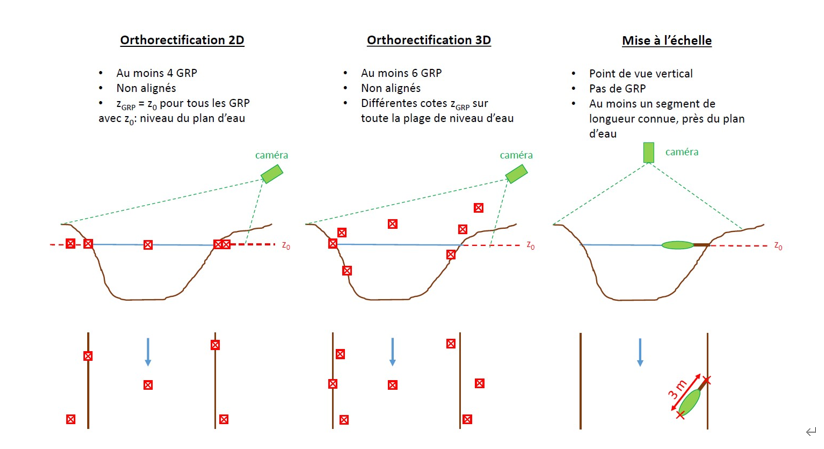
\includegraphics[width=1\linewidth,]{images/Orthowang} \caption{présentation des différents modes d'orthorectification selon la position de la caméra (source à préciser)}\label{fig:orthowang}
\end{figure}

\hypertarget{calcul-de-la-vitesse-du-duxe9placement-des-traceurs}{%
\subsection{Calcul de la vitesse du déplacement des traceurs}\label{calcul-de-la-vitesse-du-duxe9placement-des-traceurs}}

Les logiciels LSPIV calculent la vitesse instantanée de surface d'une rivière ou cours d'eau en utilisant une méthode statique en corrélation croisée, cette méthode détermine le déplacement des traceurs sur les images ortho rectifiées à condition que les traceurs soient visibles à la surface.

La méthode analyse statistiquement la position des traceurs en commun sur deux images successives séparées par un intervalle de temps. Cela consiste à calculer la corrélation entre l'aire d'interrogation \(\text{AI}\) centrée sur un point \(a_{ij}\) dans la première image, et l'aire \(\text{IA}\) centrée sur un point \(b_{ij}\) dans la deuxième image, où \(\text{IA}\) définira la taille des traceurs étudiés dans l'identification des déplacements. Le calcul des déplacements est effectué sur la deuxième image dans l'aire de recherche \(\text{SA}\) sur le point \(b_{ij}\) .



\begin{figure}[H]
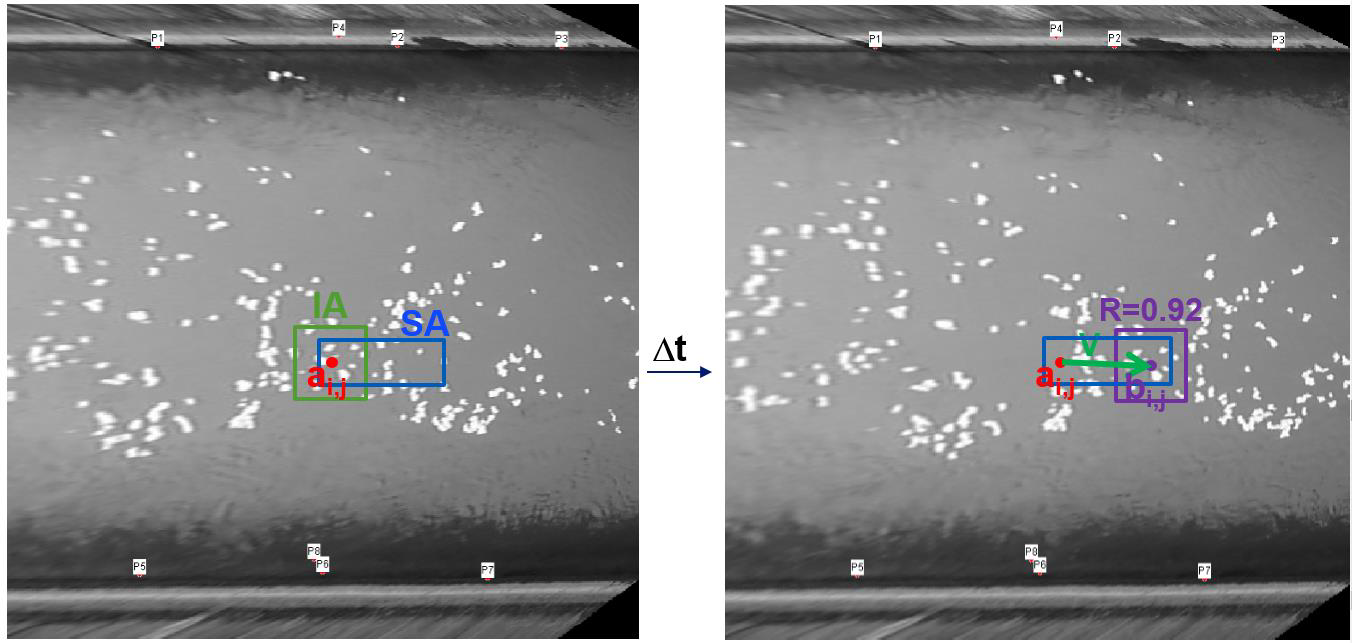
\includegraphics[width=1\linewidth,]{images/calculationdevitesse} \caption{Principe d'identification du déplacement des traceurs (Manuel d'utilisation Fudaa-LSPIV Version 1.6.4)}\label{fig:unnamed-chunk-4}
\end{figure}

\hypertarget{calcul-de-duxe9bit}{%
\subsection{Calcul de débit}\label{calcul-de-duxe9bit}}

Les logiciels LSPIV utilisent le profil bathymétrique d'une section en travers et la vitesse moyennée de profondeur pour calculer le débit dans cette section.

Les points du profil bathymétrique doivent être introduits en commençant par la berge gauche vers la berge droite ; les points aux extrémités devront être à une côte supérieure à celle de la surface de l'eau, et au moins un des points intérieurs aura une côte inferieure à la surface de l'eau.

Fudaa-LSPIV calcule la vitesse instantanée de surface à partir de traceurs, mais pour obtenir la vitesse de profondeur Fudaa-LSPIV utilisera un coefficient de vitesse \(\alpha\):

\begin{equation}
\alpha =  \frac{\text{Vitesse moyenne sur la tranche d'eau}}{\text{Vitesse de surface}}
\end{equation}

Une valeur de \(\alpha\) égale à 0.86 peut être choisie pour un écoulement moyen. La valeur de \(\alpha\) sera inférieure à 0.86 en écoulements peu profond ou rugueux, et pour les écoulements de majeur profondeur ou lisse \(\alpha\) sera supérieure à 0.86 \citep{hauet_application_2013} .

\newpage

  \bibliography{LSPIV.bib}

\end{document}
